\begin{frame}
    \begin{theorem}[Riemannsche Hypothese]
        Abgesehen von den \glqq trivialen\grqq\ Nullstellen bei $s = -2n,\; n\in \N$ haben alle Nullstellen Realteil $\frac{1}{2}$.
    \end{theorem}
    \begin{figure}
        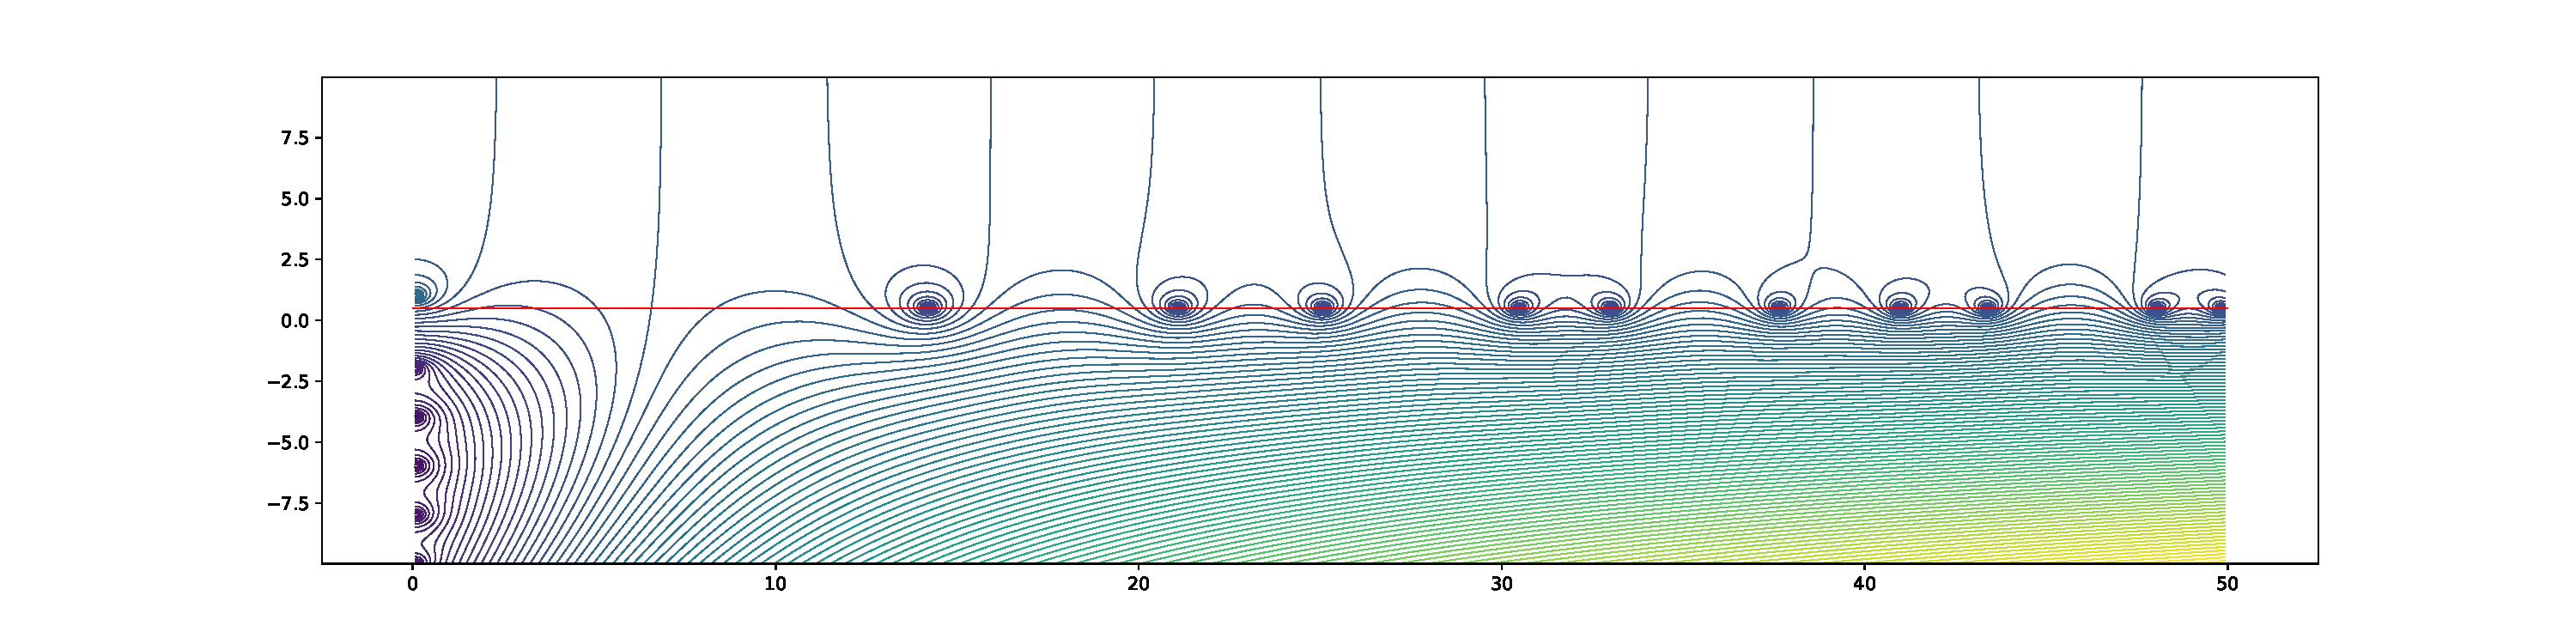
\includegraphics[trim=181 46 145 44, clip,width=\textwidth]{figures/jupyter_zeros.pdf}
        \caption{Imaginärteil der $\zeta$-Funktion bei $\Re s = \frac{1}{2}$ von $\Im s = 0$ bis $\Im s = 50$}
    \end{figure}
\end{frame}